%%%%%%%%%%%%%%%%%%%%%%%%%%%%%%%%%%%%%%%%%%%%%%%%%%%%%%%%%%
\section{Representation}
\label{sec:representation}
%%%%%%%%%%%%%%%%%%%%%%%%%%%%%%%%%%%%%%%%%%%%%%%%%%%%%%%%%%

%This section: CCG representation, including types, the grammar.
In this section, we first define our type system, then discuss our lexicon, then describe how we parse. Our system takes a three-step parsing approach. First, we use a CCG parser to build a set base parses for each temporal phrase in isolation (where each base parse is referred to a a context-independent parse). Then, for each context-independent parse, we deterministically build five context-dependent parses. Once we select a single parse from the set of candidate context-depndent parses (which we discuss in the section titled Learning), we execute the parse to ground to a final representation.

%%%%%%%%%%%%%%%%%%%%%%%%%%%%%%%%%%%%%%%%%%%%%%%%%%%%%%%%%%
\subsection{Types within CCG}
\label{sec:CCGtypes}
%%%%%%%%%%%%%%%%%%%%%%%%%%%%%%%%%%%%%%%%%%%%%%%%%%%%%%%%%%
\begin{definition}[Range]
A range is a period between two times. For example, \emph{June 13th, 2013}, \emph{today}, and \emph{1987} all ground to ranges.
\end{definition}

\begin{definition}[Sequence] 
A sequence represents an infinite sequence of ranges. For example, \emph{each Thursday} grounds to a range. The duration between each range in a sequence is the same. In the example \emph{each Thursday}, there is a week between each range. Sequences are represented as under-specified ranges. If we were interested in grounding the phrase \emph{June 13th, 2013}, we could first ground \emph{June 13th} to the sequence of all June 13ths, which we could represent as XXXX-6-13, i.e. June 13th of an unspecified year.
\end{definition}

\begin{definition}[Duration]
A duration is a period of time with no specified start or end dates. For example, \emph{two months}, \emph{three years}, and \emph{one day} all ground to durations of time. 
\end{definition}

\begin{definition}[Number]
Numbers only appear in logical forms, never in fully executed output. Numbers are necessary when grounding durations, such as \emph{4 years}, \emph{1 hour}, or \emph{3 weeks}. 
\end{definition}

\begin{definition}[Functional Types]
There are a number of functional types, all of arity less than or equal to two. They are fully outlined in a table in section TODO PUT SECTION HERE
\end{definition}

%%%%%%%%%%%%%%%%%%%%%%%%%%%%%%%%%%%%%%%%%%%%%%%%%%%%%%%%%%
\subsection{Lexicon}
%%%%%%%%%%%%%%%%%%%%%%%%%%%%%%%%%%%%%%%%%%%%%%%%%%%%%%%%%%
We use standard CCG combination rules and a hand-built lexicon to build our base parses. This approach builds upon the assumption that language is compositional in nature.

\begin{figure}[t!]
   \center
   {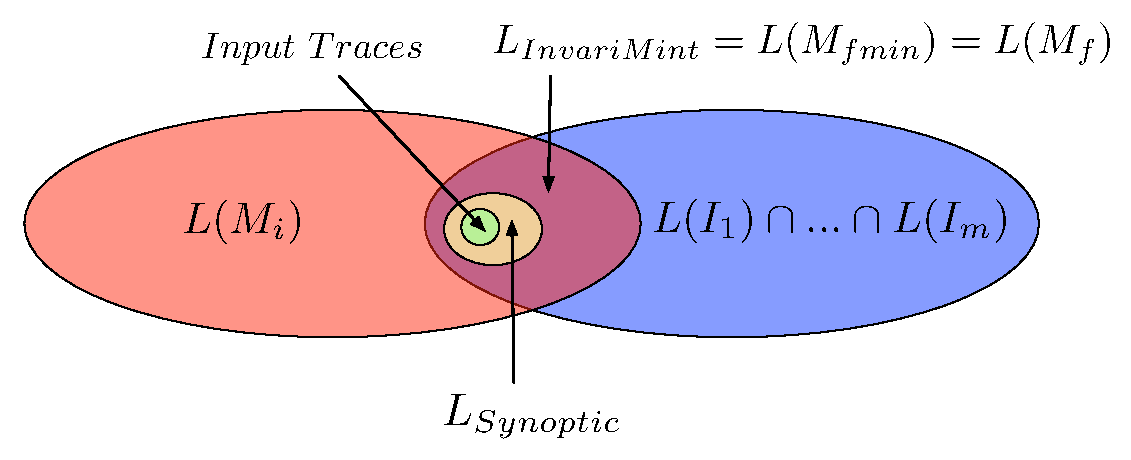
\includegraphics[width=0.95\columnwidth]{fig/language-venn.pdf}}
   \caption{This diagram illustrates the relationships between languages
    accepted by various models of the input traces. $L(M_i)$ is the language of
    the initial model which includes all of the input traces and is constrained
    only by the $NIFby$ invariants.
    $L(I_1) \cap \ldots \cap L(I_m)$ is the language of the intersected mined
    invariants. By design, $L(I_1)$ accepts all of the input traces.
    $L_{Synoptic}$ also accepts all of the input traces and is constrained by
    both the mined invariants and $M_i$. 
    Since Synoptic is non-deterministic, $L_{Synoptic}$ may vary given the same
    inputs but always respects the above constraints.
    $L_{InvariMint}$ is precisely the intersection of $L(M_i)$ and $L(I_1) \cap
    \ldots \cap L(I_m)$.
   } 
   \label{fig:language-venn}
\end{figure}


%%%%%%%%%%%%%%%%%%%%%%%%%%%%%%%%%%%%%%%%%%%%%%%%%%%%%%%%%%
\subsection{Constructing the final model}
%%%%%%%%%%%%%%%%%%%%%%%%%%%%%%%%%%%%%%%%%%%%%%%%%%%%%%%%%%

%%%%%%%%%%%%%%%%%%%%%%%%%%%%%%%%%%%%%%%%%%%%%%%%%%%%%%%%%%
\subsection{Implementation}
\label{sec:implementation}
%%%%%%%%%%%%%%%%%%%%%%%%%%%%%%%%%%%%%%%%%%%%%%%%%%%%%%%%%%

